\chapter{Effects of Network Topology}

\section{Node Distance from the Anchors}

Of great assistance to network designers would be to know in which regions of the network to expect poor localization performance.  With this information, and if the anchor placement is constrained, they could either avoid placing nodes in the expected poor area, or take into account the higher expected localization errors in the analysis of the data.

Figure~\ref{fig:AS6goodcontour} shows a different view of errors within two sample networks in attempt to find a correlation between sensor node location and each node's location error, especially based on relative location to the anchor nodes.  The plot, instead of showing a line representing the localization errors as in other figures presented in this study, the error at each node is used to interpolate a grid of location errors throughout the area of the network.  A contour plot, based on that interpolated grid, is then shown in the figure.  The anchor nodes are shown, with their radio range shown as a dashed circle.  

Figure~\ref{fig:AS6goodcontour} shows two random networks, with the same anchor node placements. In general, the region around the anchor nodes themselves has better localization performance, shown with darker color.  However, there is quite a large variability in errors throughout the network.  This simple example demonstrates that, unfortunately, no significant geographic correlation between location error and anchor node placement can be ascertained.  As shown in \ref{sec:AnchorNodeError}, the localization error has almost no correlation with the density of nodes around anchor nodes or the error of the anchor nodes themselves.  Therefore, the lack of correlation of any sensor node's location relative to the anchor nodes is not surprising.

However, there are likely other factors, such as network density, algorithm parameters to the underlying localization protocol of CCA-MAP, or yet undiscovered factors, that may be masking any it may be possible, correlation to the location of a sensor node relative to the anchor nodes.  Therefore, with future study, it may be possible to remove the effect of these other factors to reveal a pattern based on anchor placement. 

\begin{figure}
  \centering
	\subfloat[Network A]{
		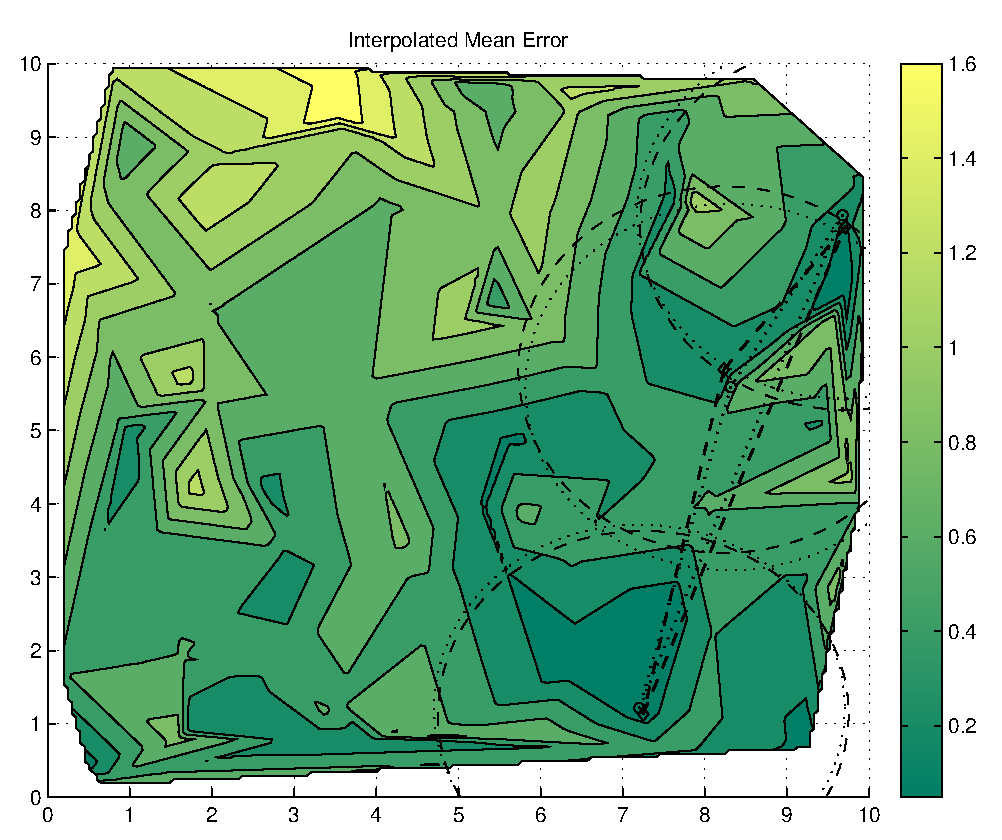
\includegraphics[width=\figurewidth\textwidth]{outliers/AS6/AS6NetworkContour7}}
	\\
	\subfloat[Network B]{
		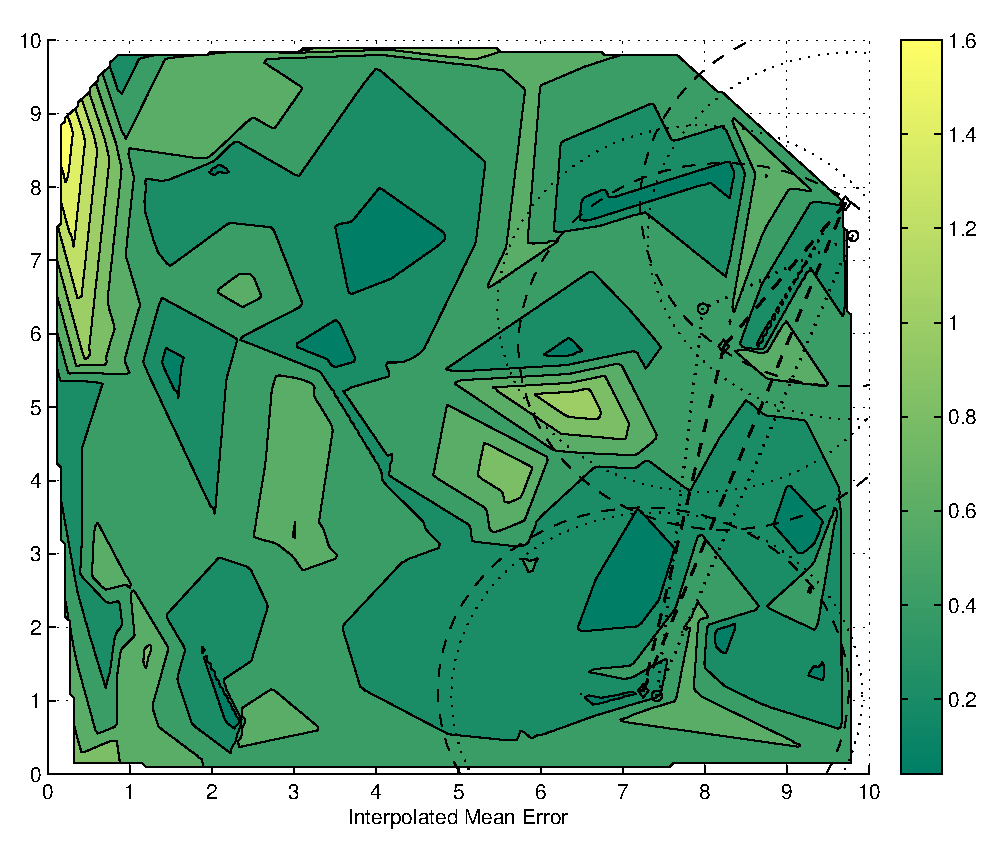
\includegraphics[width=\figurewidth\textwidth]{outliers/AS6/AS6NetworkContour10}}
	\caption{Localization error as a contour plot}
	\label{fig:AS6goodcontour}
\end{figure}

\section{Applicability to Varying Network Topologies}

So far, we have examined anchor node placement for a continuous square network, with randomly placed nodes.  However, in the real world, networks are not alway so simple.  There are often regions in the network where it is not possible to put nodes, due to physical barriers like lake, buildings or access to property.  In this section, we look at how the results thus far apply to C-shaped and long, narrow pipeline network topologies.

\subsection{C-Shape Network Topology}

A C-shape network consists of a relatively square region with an empty area on one side, as shown in Figure~\ref{fig:cnetwork}.  In terms of anchor placement requirements, we do not expect any difference between the recommendations presented for square networks.

\begin{figure}
  \centering
	\includegraphics[width=\textwidth]{cshape/network}
	\caption{Example of C-shape network topology}
	\label{fig:cnetwork}
\end{figure}

To show that there is no difference between C-shape and square network topologies, 10 random C-shape networks with 5,000 anchor sets each were simulated in the same manner as the square networks.  Figure~\ref{fig:cshapesum} shows the location error relative to the sum of the distances between the anchors, as in Section~\ref{sec:bestanchornode}.  As expected, the mean location error flattens out as the sum of distances between anchor nodes reaches about 10 times the radio range as was the case with the square network.  There is a slight increase in the floor of the mean location error as compared with the square network, but this has to do with the performance of the CCA algorithm in the presence of the empty region of nodes in the network.  The increase in mean location error at the end of the plot, and specifically the increase in the confidence interval, is caused by the small sample size in the random selection of anchor set with a very high distance between nodes.
 
Similarly, the same criteria for eliminating the outlier localization results also holds for C-shape topology as it did for square in Section~\ref{sec:outlierindicators}.  Figure~\ref{fig:cshapeheight} shows that as long as the minimum height of the triangle formed by the anchors nodes is greater than the radio range, then the outlier case can be avoided, as is the case for a square network.

\begin{figure}
  \centering
	\subfloat[Sum of distance between anchors vs. mean location error, excluding outliers]{\label{fig:cshapesum}
		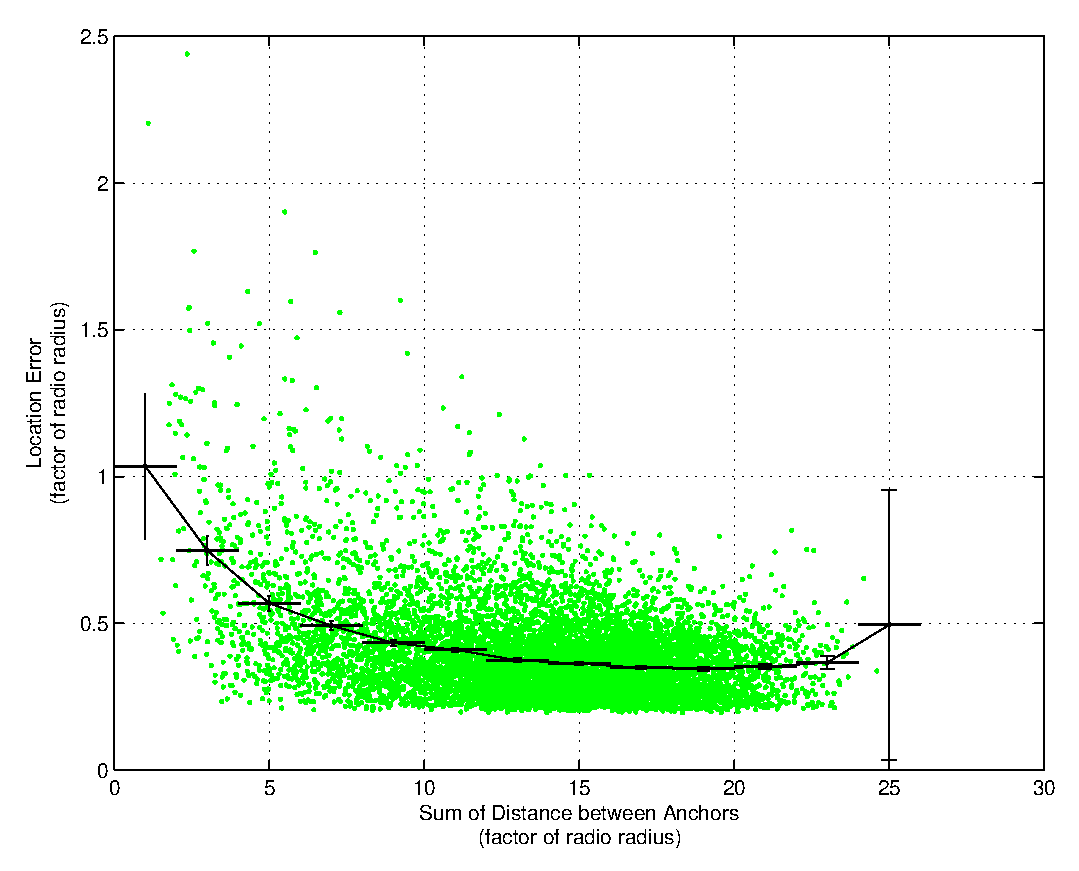
\includegraphics[width=\figurewidth\textwidth]{cshape/SumOfDistanceIndicator_cshape}}
	\\
	\subfloat[Minimum height of anchor triangle vs. mean location error]{\label{fig:cshapeheight}
		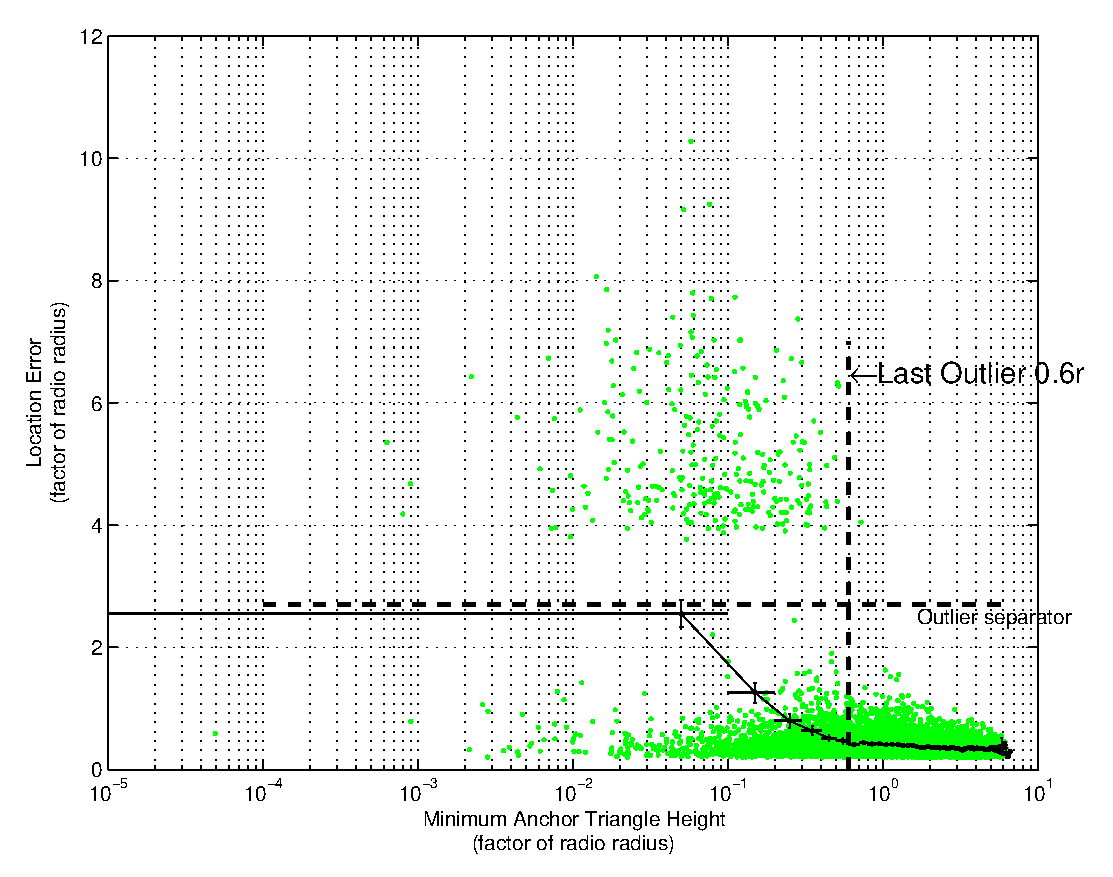
\includegraphics[width=\figurewidth\textwidth]{cshape/HeightIndicator_cshape}}
	\caption[Anchor metrics for a C-Shape topology]{Anchor metrics for 10 random C-shape 20-by-20 unit networks with 400 nodes, 5,000 anchor sets each, and a radio range of 2.5 units}
	\label{fig:cindicator}
\end{figure}

\subsection{Pipeline Network Topology}

In some applications, the network region has very little depth to it, such as when monitoring a gas pipeline or along a highway or railroad line.  The extreme case is where there is a single node placed along a straight axis.  As we have shown, this is the worst possible scenario, as it is the most likely way to cause the outlier condition for localization.  In that case, it is worthwhile to explore the possibility of other localization techniques, such as GPS at each node, or recording the location as the nodes are placed.

However, when there is a bit of depth to the network, as shown in Figure~\ref{fig:pipeline}, there is still the possibility of good localization results.  To demonstrate the importance of having an anchor node triangle height of at least the radio range, Figures~\ref{fig:pipessum} and \ref{fig:pipesheight} show mean location error for four different networks, with increasing network depth, but the same length.  

\begin{figure}
  \centering
	\includegraphics[width=\textwidth]{pipeline/network}
	\caption{Example of pipeline network topology}
	\label{fig:pipeline}
\end{figure}

As before, we attempt to distinguish the outlier case with a plot of the sum of distance between anchors. Figure~\ref{fig:pipessum} shows that as the network has a larger depth, the floor of possible localization errors drops.  In particular, when the network depth is only 1, the floor is about 0.5r, whereas when the depth is 4 units, or twice the radio range, the floor drops to roughly 0.25r.  Also, as the sum of the distance increases and the network depth is greater than the radio range, the outlier cases become apparent.  

\begin{figure}
  \centering
	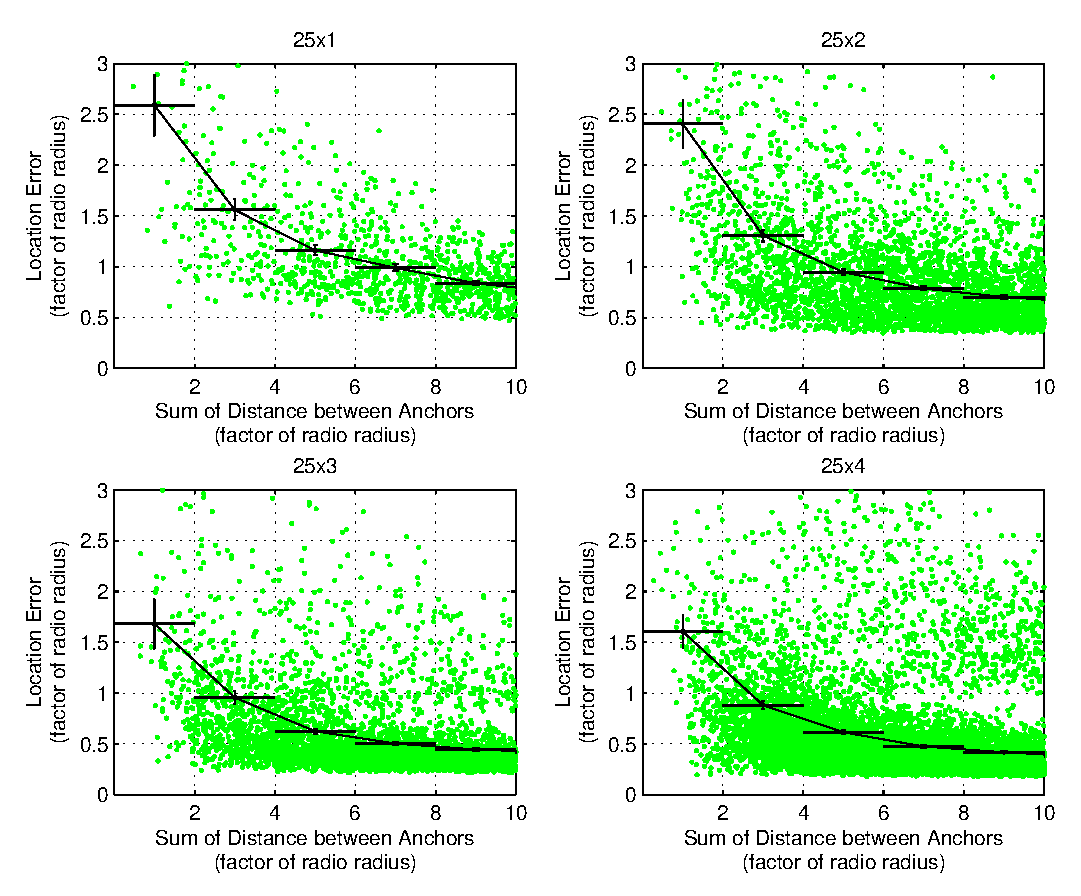
\includegraphics[width=\textwidth]{pipeline/SumOfDistanceIndicator_pipes}
	\caption[Sum of distance between anchors vs. mean location error]{Sum of distance between anchors vs. mean location error for random pipeline 25-by-1,2,3 and 4 unit networks with 200 nodes, 1,000 anchor sets each, and a radio range of 2.0 units}
	\label{fig:pipessum}
\end{figure}

Interestingly, the outlier cases have a much lower mean localization error in a pipeline topology.  Figure~\ref{fig:pipesspread} shows two sample anchor sets that demonstrate the difference in localization performance when the anchors are clumped together versus spread apart.  When the anchor nodes are clumped together, the calculated positions remain in a straight line, as the expected results do, but the algorithm cannot determine the correct angle that line should take.  However, since the lines do cross where the anchor nodes are clumped, the line is grounded to a relatively accurate level, when compared with the square networks. For this reason, the outlier case, in general, has lower error in a pipeline topology. Nonetheless, it is poor performance, and is likely not useful in most applications.

\begin{figure}
  \centering
	\subfloat[Pipeline with spread apart anchors]{\label{fig:pipelinespread}
		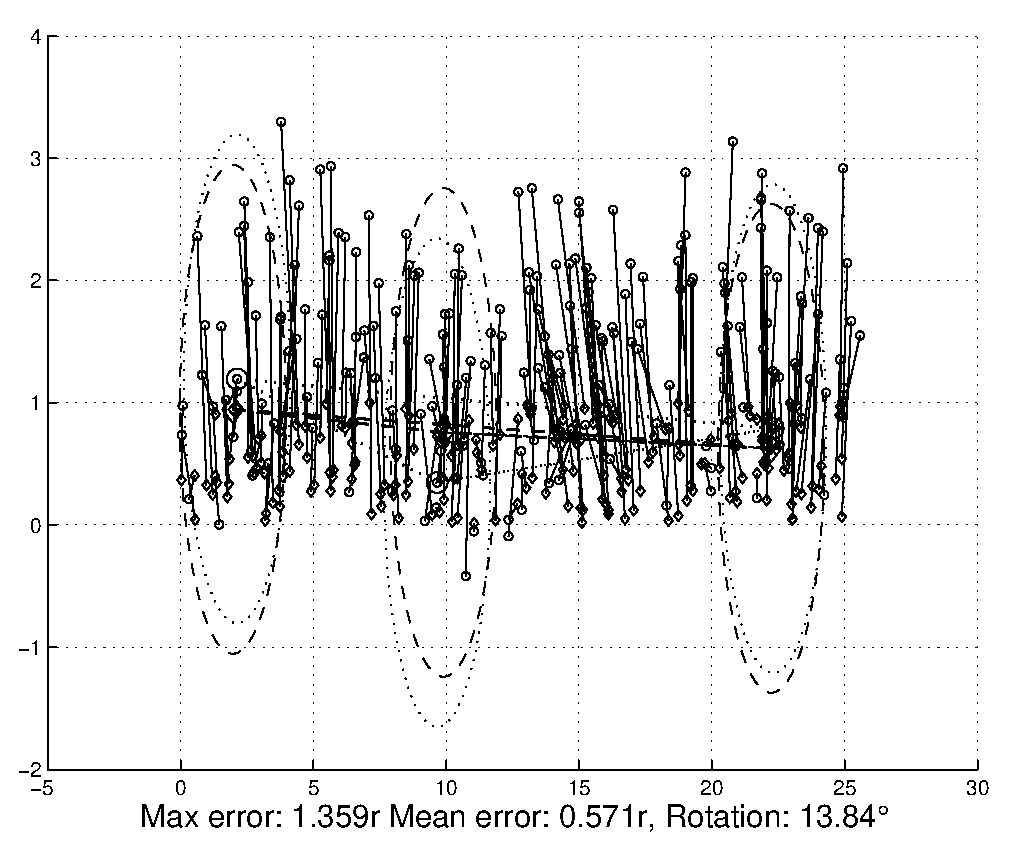
\includegraphics[width=\figurewidth\textwidth]{pipeline/spread}}
	\\
	\subfloat[Pipeline with clumped anchors]{\label{fig:pipelineclumped}
		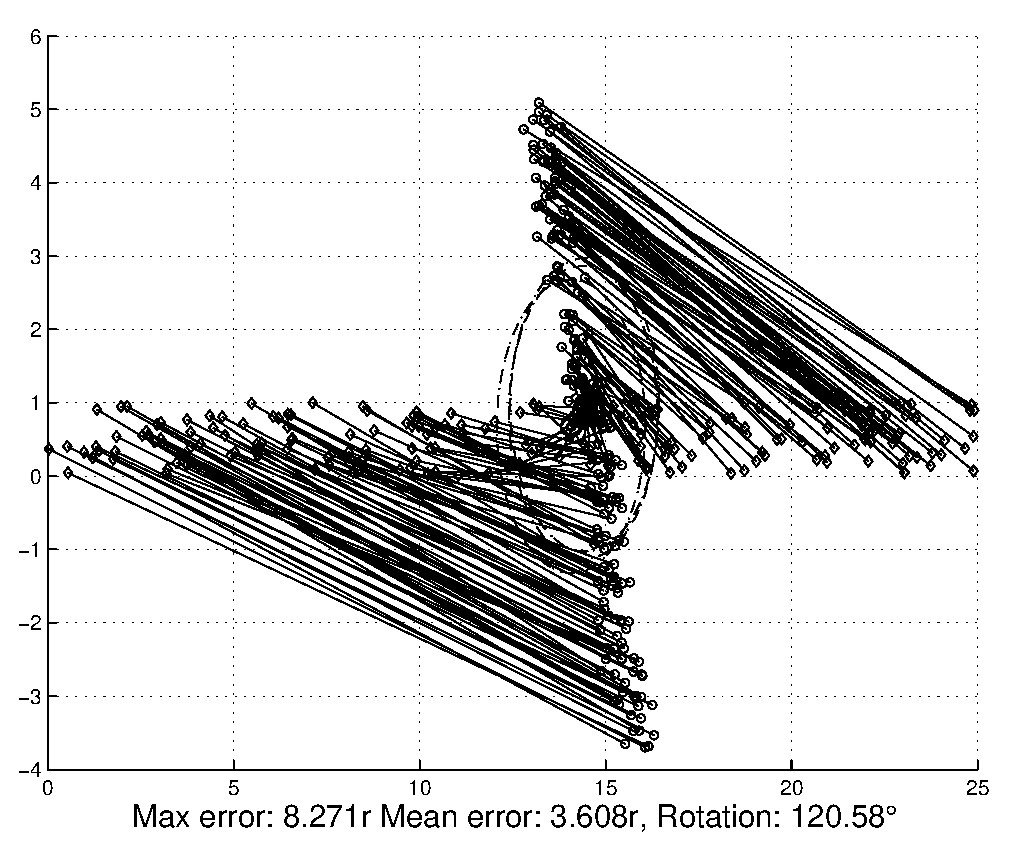
\includegraphics[width=\figurewidth\textwidth]{pipeline/clumped}}
	\caption{Pipeline network with anchors spread apart and clumped together}
	\label{fig:pipesspread}
\end{figure}

The plots of minimum triangle height in Figure~\ref{fig:pipesheight} show that for networks with a depth less than the radio range, the separation of good and outlier cases is impossible to distinguish.  Specifically, when the network depth is 1 units, half the radio range, the mean localization error is basically flat across all triangle heights possible.  As it becomes possible to have anchor sets forming a triangle with height more than the radio range, localization performance drops down to normal levels, below 0.5r, when the triangle height is also greater than the radio range.  However, the minimum triangle height no longer appears to be a good indicator of outlier cases. 

\begin{figure}
  \centering
	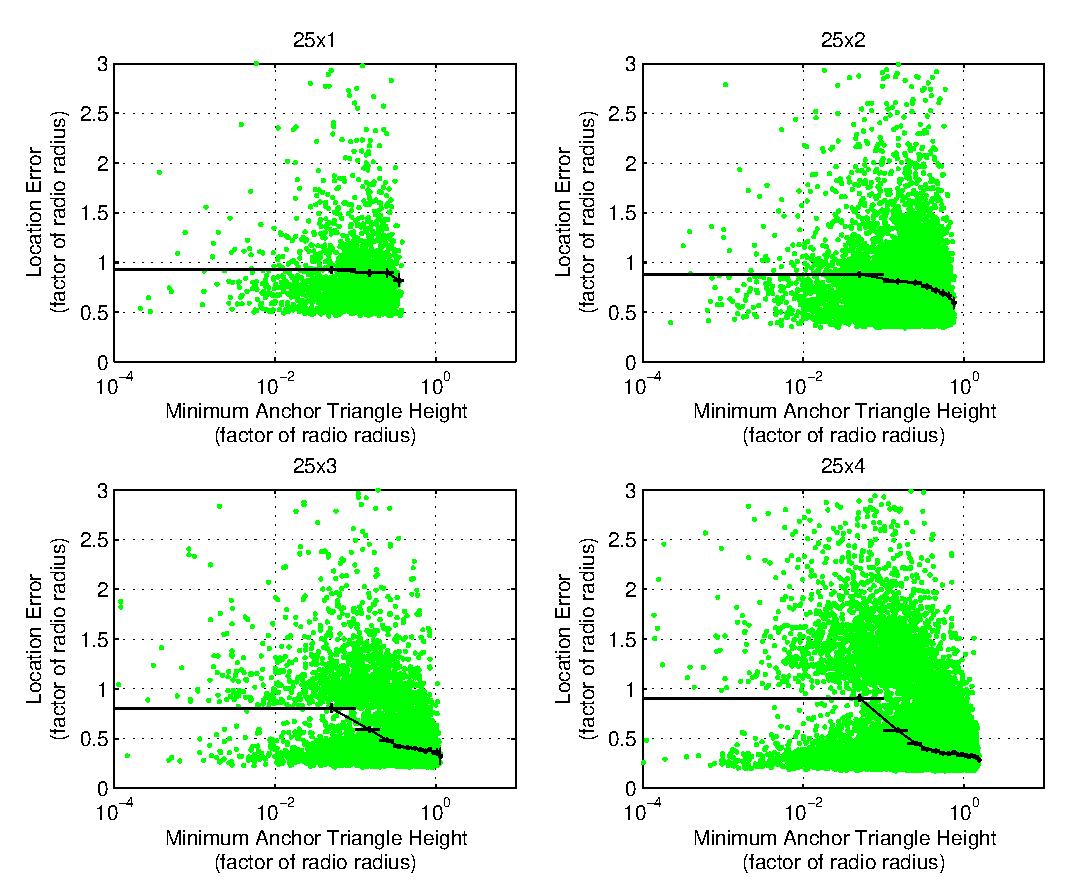
\includegraphics[width=\textwidth]{pipeline/HeightIndicator_pipes}
	\caption[Minimum height of anchor triangle vs. mean location error]{Minimum height of anchor triangle vs. mean location error for random pipeline 25-by-1,2,3 and 4 unit networks with 200 nodes, 1,000 anchor sets each, and a radio range of 2.0 units}
	\label{fig:pipesheight}
\end{figure}

In the end, even though the results are better when the depth of the pipeline is more than the radio range, it is impossible to reliably avoid the outlier condition.  Therefore, for a pipeline topology, we recommend to use a different class of localization algorithms that does not rely on transforming local coordinates into global coordinates with anchor nodes.  If no other algorithms are possible, we recommend making the network as deep as possible and to spread the anchors as apart along the length of the pipeline as possible.  

